\startcontents[localtoc]
\printcontents[localtoc]{}{0}{\subsection*{Contents}\setcounter{tocdepth}{2}}



\phantomsection
\addcontentsline{toc}{section}{Generate simple sine waveform}
\subsubsection*{Generate simple sine waveform}



Consider we want to simulate a sampled voltage waveform with frequency 1,
amplitude 1, phase 1 and offset 1. The waveform was sampled with sampling
frequency 1 kHz and number of samples was 1000. The waveform contains also
3rd harmonic with amplitude of 0.1 V, and noise at level 1 mV.

\begin{lstlisting}
DI = [];
DI.fs.v = 1e3;
DI.L.v = 1e3;
DI.f.v = [1 3];
DI.A.v = [1 0.1];
DI.ph.v = [0 pi];
DI.O.v = [0 0];
DI.noise.v = 0.001;
DO = qwtb('GenNHarm', DI);
\end{lstlisting}
\begin{lstlisting}[language={},xleftmargin=5pt,frame=none]
QWTB: no uncertainty calculation
QWTB: GenNHarm wrapper: time series was calculated from sampling frequency and number of samples.
QWTB: GenNHarm wrapper: time series was calculated from number of samples.

\end{lstlisting}


\phantomsection
\addcontentsline{toc}{section}{Calculated THD\_k1}
\subsubsection*{Calculated THD\_k1}



The output structure contains the calculated value of the THD\_k1 quantity:

\begin{lstlisting}
DO.thd_k1.v
\end{lstlisting}
\begin{lstlisting}[language={},xleftmargin=5pt,frame=none]
ans = 0.1000

\end{lstlisting}


\phantomsection
\addcontentsline{toc}{section}{Plot}
\subsubsection*{Plot}



The generated waveform:

\begin{lstlisting}
figure
plot(DO.t.v, DO.y.v, '-');
xlabel('t (s)'), ylabel('amplitude (V)')
\end{lstlisting}
\begin{center}
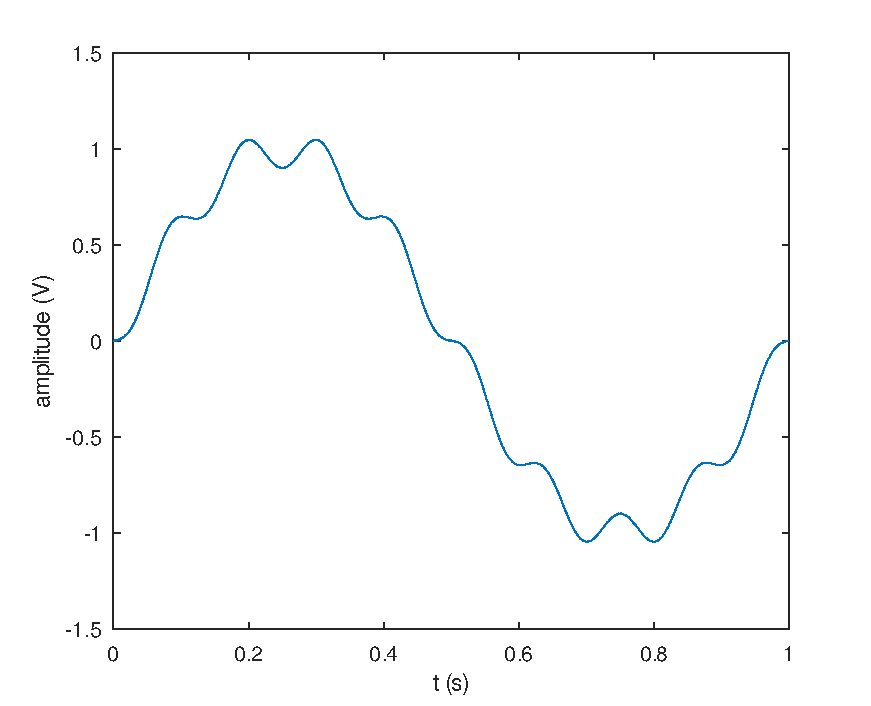
\includegraphics[width=0.7\textwidth]{algs_examples_published/GenNHarm_alg_example-1.pdf}
\end{center}


\phantomsection
\addcontentsline{toc}{section}{Generate simple sine waveform using number of periods}
\subsubsection*{Generate simple sine waveform using number of periods}



Consider we want to simulate 2.5 periods of a sine waveform.

\begin{lstlisting}
DI = [];
DI.fs.v = 1e3;
DI.M.v = 2.5;
DI.f.v = [1];
DI.A.v = [1];
DI.ph.v = [0];
DI.O.v = [0];
DI.noise.v = 0;
DO = qwtb('GenNHarm', DI);
figure
plot(DO.t.v, DO.y.v, '-');
xlabel('t (s)'), ylabel('amplitude (V)')
\end{lstlisting}
\begin{lstlisting}[language={},xleftmargin=5pt,frame=none]
QWTB: no uncertainty calculation
QWTB: GenNHarm wrapper: time series was calculated from sampling frequency and number of samples.
QWTB: GenNHarm wrapper: time series was calculated from number of main signal component periods.

\end{lstlisting}
\begin{center}
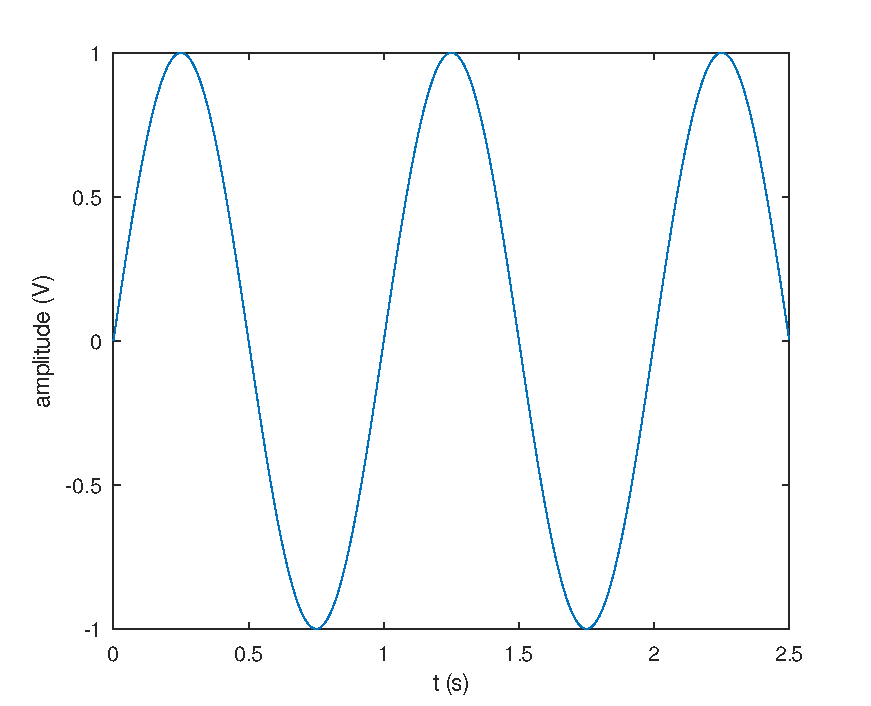
\includegraphics[width=0.7\textwidth]{algs_examples_published/GenNHarm_alg_example-2.pdf}
\end{center}


\phantomsection
\addcontentsline{toc}{section}{Generate waveform with automatically calculated harmonics}
\subsubsection*{Generate waveform with automatically calculated harmonics}



Consider waveform with 10 harmonic components, while the amplitudes of the
harmonics will be calculated based on the supplied THD\_k1 value. The \texttt{f},
\texttt{A}, \texttt{ph} and \texttt{O} quantities will contain only values for first harmonic. The
rest harmonics will be added by the waveform generator.

\begin{lstlisting}
DI = [];
DI.fs.v = 1e3;
DI.L.v = 1e3;
DI.f.v = [1];
DI.A.v = [1];
DI.ph.v = [0];
DI.O.v = [0];
DI.thd_k1.v = 0.1;
DI.nharm.v = 9;
DO = qwtb('GenNHarm', DI);
figure
plot(DO.t.v, DO.y.v, '-')
xlabel('t (s)'), ylabel('amplitude (V)')
\end{lstlisting}
\begin{lstlisting}[language={},xleftmargin=5pt,frame=none]
QWTB: no uncertainty calculation
QWTB: GenNHarm wrapper: time series was calculated from sampling frequency and number of samples.
QWTB: GenNHarm wrapper: time series was calculated from number of samples.

\end{lstlisting}
\begin{center}
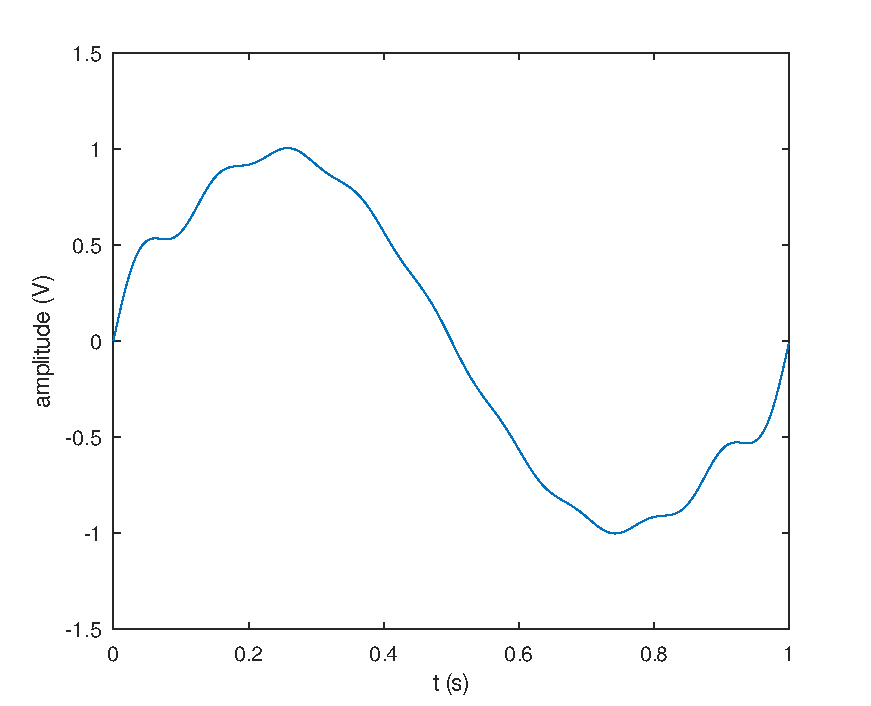
\includegraphics[width=0.7\textwidth]{algs_examples_published/GenNHarm_alg_example-3.pdf}
\end{center}


\phantomsection
\addcontentsline{toc}{section}{Check using FFT}
\subsubsection*{Check using FFT}



We can check the generated waveform by calculating the spectrum. Output of GenNHarm will be used as input into the algorithm \texttt{SP-WFFT}.

\begin{lstlisting}
DIspec = DO;
DIspec.fs.v = DI.fs.v;
DOspec = qwtb('SP-WFFT', DIspec);
figure
semilogy(DOspec.f.v, DOspec.A.v, 'o');
xlim([-2 12]); ylim([1e-3 10]);
\end{lstlisting}
\begin{lstlisting}[language={},xleftmargin=5pt,frame=none]
QWTB: no uncertainty calculation
warning: axis: omitting non-positive data in log plot
warning: called from
    __plt__>__plt2vv__ at line 502 column 10
    __plt__>__plt2__ at line 248 column 14
    __plt__ at line 115 column 16
    semilogy at line 65 column 10
    publish>eval_code_helper at line 1079 column 8
    publish>eval_code at line 995 column 30
    publish at line 402 column 9
    all_algs_examples2tex at line 51 column 5
 

\end{lstlisting}
\begin{center}
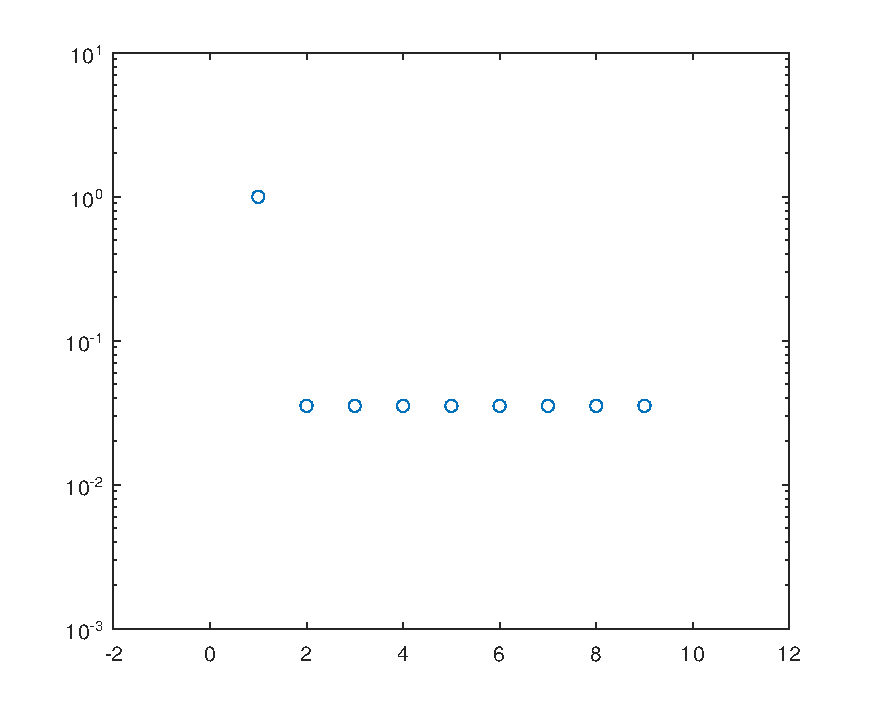
\includegraphics[width=0.7\textwidth]{algs_examples_published/GenNHarm_alg_example-4.pdf}
\end{center}


\stopcontents[localtoc]
